\chapter*{2019年\textsf{HDU}「大学物理1」期中试题解答}

\begin{minipage}{0.32\textwidth}
    \textbf{开课学院}：理学院
      
    \textbf{课程编码}：A0715011
\end{minipage}
\hfill
\begin{minipage}{0.32\textwidth}
    \textbf{解析制作}：\textsf{M.Xia@WeYoung}

    \textbf{\,\hologo{TeX}~排版}：\textsf{M.Xia}
\end{minipage}
\hfill
\begin{minipage}{0.15\textwidth}
    \centering
    \begin{tikzpicture}
        \node [inner sep=0] at (0,0) {
            \qrcode[height=3em,version=4]{https://qm.qq.com/q/mgD30uPiSs}};
        \fill [color=white,rounded corners=(sqrt(2)+2)/11*1em] (-.5em,-.5em) rectangle (.5em,.5em);
        \node [inner sep=0] at (0,0) {\color{MidnightBlue}\scriptsize\faIcon{qq}};
    \end{tikzpicture}

    \scriptsize\href{https://qm.qq.com/q/mgD30uPiSs}{\itshape 未央物理营}
\end{minipage}
\hfill
\begin{minipage}{0.15\textwidth}
    \centering
    \begin{tikzpicture}
        \node [inner sep=0] at (0,0) {
            \qrcode[height=3em,version=4]{http://weixin.qq.com/r/DBIABcHEqgnWKIVmb0eI}};
            \fill [color=white,rounded corners=(sqrt(2)+2)/11*1em] (-.5em,-.5em) rectangle (.5em,.5em);
        \node [inner sep=0] at (0,0) {\color{DarkGreen}\scriptsize\faIcon{weixin}};
    \end{tikzpicture}

    \scriptsize\href{http://weixin.qq.com/r/DBIABcHEqgnWKIVmb0eI}{\itshape 未央学社}
\end{minipage}

\section{选择题（每题3分，共30分）}

\begin{problem}
    以下几种运动形式中，$\bm a$保持不变的运动
    \begin{tasks}(4)
        \task 单摆的运动
        \task[\true] 抛体运动
        \task 匀速率圆周运动
        \task 行星椭圆运动
    \end{tasks}
\end{problem}
\begin{solution}
    C选项中加速度的方向会发生改变，A、D选项中加速度的大小和方向都会发生改变.
\end{solution}

\begin{problem}
    一质点作直线运动，某时刻的瞬时速度$v=\qty2{\m/\s}$，瞬时加速度$a=\qty{-2}{\m\cdot\s^{-2}}$，则一秒钟后质点的速度
    \begin{tasks}(4)
        \task 等于零
        \task 等于$\qty{-2}{\m/\s}$
        \task 等于$\qty2{\m/\s}$
        \task[\true] 不能确定
    \end{tasks}
\end{problem}
\solute2
\begin{solution}
    由于题目中未强调质点的加速度是否为常数，所以一秒钟后质点的速度不能确定.
\end{solution}

\begin{problem}
    \begin{paracol}{2}
    光滑的水平桌面上放有两块相互接触的滑块，质量分别为$m_1$和$m_2$，且$m_1<m_2$. 今对两滑块施加相同的水平作用力，如图所示. 设在运动过程中，两滑块不离开，则两滑块之间的相互作用力$N$应有
    \switchcolumn\vspace*{\fill}\centering
    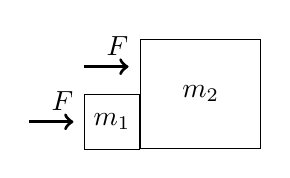
\begin{tikzpicture}[scale=.7]
        \wall{(-3,.02)}{(2.5,-.2)};
        \draw (-2,0) rectangle (-1,1) node [midway] {$m_1$};
        \draw (-.98,.02) rectangle (1.2,2) node [midway] {$m_2$};
        \draw [very thick,->] (-3,.5) -- (-2.2,.5) node [above,near end] {$\bm F$};
        \draw [very thick,->] (-2,1.5) -- (-1.2,1.5) node [above,near end] {$\bm F$};
    \end{tikzpicture}\vspace*{\fill}
\end{paracol}
    \begin{tasks}(4)
        \task $N=0$
        \task $F<N<2F$
        \task[\true] $0<N<F$
        \task $N>2F$
    \end{tasks}
\end{problem}
\solute4
\begin{solution}
    两滑块相互接触且加速度相等但$m_1<m_2$，所以必存在挤压，$N>0$. 如果二者之间的作用力等于$F$，则$m_1$所受合外力为零，加速度为零. 所以二者之间的作用力$N$满足$0<N<F$.
\end{solution}

\begin{problem}
    已知水星的半径是地球半径的$0.4$倍，质量为地球的$0.04$倍. 设在地球上的重力加速度为$g$，则水星表面上的重力加速度为
\begin{tasks}(4)
\task[\true] $0.25g$
\task $0.1g$
\task $2.5g$
\task $4g$
\end{tasks}
\end{problem}
\solute2
\begin{solution}
    由引力提供重力$GMm/R^2=mg$得$g=GM/R^2\propto M/R^2$. 由于水星的半径是地球半径的$0.4$倍，质量为地球的$0.04$倍，所以其表面上的重力加速度为$g'=0.04/0.4^2\times g=0.25g$.
\end{solution}

\begin{problem}
    有两个半径相同，质量相等的细圆环$A$和$B$. $A$环的质量分布均匀，$B$环的质量分布不均匀. 它们对通过环心并与环面垂直的轴的转动惯量分别为$I_A$和$I_B$，则
\begin{tasks}(13)
    \task*(3) $I_A>I_B$
    \task*(3) $I_A<I_B$
    \task*(3)[\true] $I_A=I_B$
    \task* 不能确定$I_A$、$I_B$哪个大
\end{tasks}
\end{problem}
\solute3
\begin{solution}
    由于圆环上各点与环心处转轴的距离相同，根据转动惯量的定义，$r_i^2$项可从求和中单独提取出来，导致这种情况下转动惯量与质量分布无关，即$I=\sum{m_ir_i^2}=R^2\sum{m_i}=MR^2$.
\end{solution}

\begin{paracol}{2}
\begin{problem}
    均匀细棒$OA$可绕通过其一端$O$而与棒垂直的水平固定光滑轴转动，如图所示. 今使棒从水平位置由静止开始自由下落，在棒摆动到竖直位置的过程中，角动量$L$与角加速度$\beta$的变化趋势分别为
    \begin{tasks}(2)
    \task $L$减小，$\beta$减小
    \task $L$减小，$\beta$增大
    \task $L$增大，$\beta$增大
    \task[\true] $L$增大，$\beta$减小
    \end{tasks}
    \switchcolumn\vspace*{\fill}\centering
    \begin{tikzpicture}[scale=.8]
        \wall{(-.8,.25)}{(.8,.4)};
        \draw (-.1,-4.2) rectangle + (.2,4);
        \draw [dashed] (-.1,-.4) rectangle +(4,.2);
        \draw [rounded corners=3pt] (-.3,.25) -- (0,-.4) -- (.3,.25);
        \filldraw (0,-.3) circle (.05);
        \node [below left] at (0,-.3) {$O$};
        \node [anchor=west] at (3.9,0) {$A$};
    \end{tikzpicture}\vspace*{\fill}
\end{problem}
\end{paracol}
\solute2
\begin{solution}
    下落过程中，细棒的角速度不断增大，所以其角动量由小到大；刚释放时，其所受重力矩为$mgl/2$，摆动到竖直位置时，其所受重力矩为零，所以其角加速度由大到小.
\end{solution}

\begin{paracol}{2}
    \begin{problem}
        今有一劲度系数为$k$的轻弹簧，竖直放置，下端悬一质量为$m$的小球，开始时使弹簧为原长而小球恰好与地接触，今将弹簧上端缓慢地提起，直到小球刚能脱离地面为止，在此过程中外力做功为
        \begin{tasks}(4)
            \task[\true] $m^2g^2/2k$
            \task $m^2g^2/3k$
            \task $m^2g^2/4k$
            \task $2m^2g^2/k$
        \end{tasks}
        \switchcolumn\vspace*{\fill}\centering
        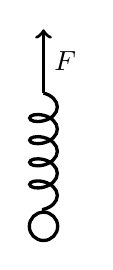
\begin{tikzpicture}[scale=.9]
            \wall{(-1.5,0)}{(1.5,-.2)};
            \draw [very thick] (0,.22) circle (.2);
            \draw [very thick,decoration={aspect=.6, segment length=8, amplitude=5,coil},decorate] (0,2.1) -- (0,.42); %amplitude调整螺线管的直径，segment length调整间距
            \draw [very thick,->] (0,2.1) -- (0,3) node [midway,right] {$F$};
        \end{tikzpicture}\vspace*{\fill}
    \end{problem}
\end{paracol}
\solute1
\begin{solution}
    小球刚脱离地面时，弹簧拉力等于小球重力，即$mg=k\Delta x$；拉力$F$做功等于弹簧弹性势能增量，即$W=k\Delta x^2/2=m^2g^2/2k$.
\end{solution}

\begin{problem}
    已知一高斯面所包围的体积内电量代数和$\sum{q_i}=0$，则可肯定
    \begin{tasks}(2)
        \task 高斯面上各点场强均为零
        \task 穿过整个高斯面的电通量为零
        \task 穿过高斯面上每一面元的电通量均为零
        \task 以上说法都对
    \end{tasks}
\end{problem}
\solute1
\begin{solution}
    高斯面所包围的体积内电量代数和为零，只能说明高斯面所包围的体积内电量代数和为零，但并不代表穿过高斯面上每一面元的电通量均为零，因为高斯面上各点场强方向可指向高斯面外，也可指向高斯面内，所以A、C选项错误.
\end{solution}

\begin{paracol}{2}
    \begin{problem}
        如图所示，在点电荷$+q$电场中，若取图中$P$点处为电势零点，则$M$点的电势为
        \begin{tasks}(4)
            \task[\true] $-q/8\pi\epsilon_0a$
            \task $q/8\pi\epsilon_0a$
            \task $-q/4\pi\epsilon_0a$
            \task $q/4\pi\epsilon_0a$
        \end{tasks}
    \end{problem}
    \switchcolumn\vspace*{\fill}\centering
    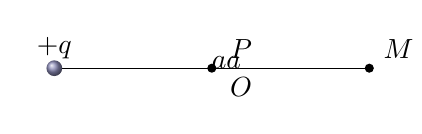
\begin{tikzpicture}
        \draw (-2,0) -- (2,0);
        \shade [ball color=MidnightBlue!50] (-2,0) circle (.1);
        \node [anchor=south] at (-2,0) {$+q$};
        \filldraw (0,0) circle (.05);
        \filldraw (2,0) circle (.05);
        \length{(-2,-1)}{(0,-1)}{$a$}{(.5,0)};
        \length{(0,-1)}{(2,-1)}{$a$}{(.5,0)};
        \node [anchor=north] at (0,0) {$O$};
        \node [anchor=south] at (0,0) {$P$};
        \node [anchor=south] at (2,0) {$M$};
    \end{tikzpicture}\vspace*{\fill}
\end{paracol}
\solute3
\begin{solution}\leavevmode
    \begin{itemize}
        \item 正常情况下，$P$点、$M$点的电势分别为$\varphi_P=q/4\pi\epsilon_0a$，$\varphi_M=q/8\pi\epsilon_0a$.
        \item 取图中$P$点为电势零点，图中所有点的电势都要减去$P$点原来的电势，此时$\varphi_P'=0$.
        \item 所以$M$点的电势为$\varphi_M'=\varphi_M-\varphi_P=-q/8\pi\epsilon_0a$.
    \end{itemize}
\end{solution}

\section{填空题（每题3分，共21分）}

\begin{problem}
    一质点沿$x$方向运动，其加速度随时间变化关系为$a=3+2t$ (SI). 如过初始时质点的速度$v_0=\qty5{\m/\s}$，则当$t$为$\qty3{\s}$时，质点的速度$v=$\ans{$\qty{23}{\m/\s}$}.
\end{problem}
\solute2
\begin{solution}
    $v=v_0+\int_0^3a\d t=v_0+\int_0^3(3+2t)\d t=\qty{23}{\m/\s}$.
\end{solution}

\begin{problem}
    一个力$F$作用在质量为$\qty{1.0}\kg$的质点上，使之沿$x$轴运动. 已知在此力作用下质点的运动学方程为$x=3t-2t^2+t^3$ (SI). 在$0$到$\qty3{\s}$的时间间隔内，力$F$对质点所作的功$W=$\ans{$\qty{157.5}\J$}.
\end{problem}
\solute3
\begin{solution}
    $W=\int_0^3{F\d x}=\int_0^3{m\ddot x\dot x\d t}=\int_0^3\qty1\kg\cdot(-4+6t)\cdot(3-4t+3t^2)\d t=\qty{157.5}\J$
\end{solution}

\begin{problem}
    一质量$m=\qty{10}\g$的子弹，以速率$v_0=\qty{500}{\m/\s}$沿水平方向射穿一物体. 穿出时，子弹的速率为$v=\qty{30}{\m/\s}$，仍是水平方向. 则子弹在穿透过程中所受的冲量的大小为\ans{$\qty{4.7}{\N\cdot\s}$}，方向为\ans{与速度方向相反}.
\end{problem}
\solute3
\begin{solution}
    $I=mv-mv_0=\qty{-4.7}{\N\cdot\s}$，负号表示方向与速度方向相反.
\end{solution}

\begin{problem}
    半径为$R$具有光滑轴的定滑轮边缘绕一细绳，绳的下端挂一质量为$m$的物体. 绳的质量可以忽略，绳与定滑轮之间无相对滑动. 若物体下落的加速度为$2a$，则定滑轮对轴的转动惯量$I=$\ans{$m(g-2a)R^2/2a$}.
\end{problem}
\solute4
\begin{solution}
    对物块列牛顿运动定律、对滑轮列转动定律，并由线量与角量之间的关系得
    \[
    \begin{dcases}
        T-mg=m\cdot 2a\\
        TR=I\beta\\
        2a=R\beta
    \end{dcases}\Longrightarrow I=\frac{m(g-2a)R^2}{2a}
    \]
\end{solution}

\begin{paracol}{2}
\begin{problem}
    如图所示，在场强为$\bm E$的均匀电场中取一半球面，其半径为$R$，电场强度的方向与半球面的对称轴平行. 则通过这个半球面的电通量为\ans{$E\pi R^2$}.
    \switchcolumn\vspace*{\fill}\centering
    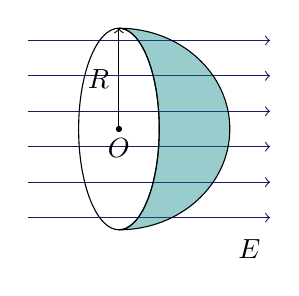
\begin{tikzpicture}[scale=.64]
        \foreach \y in {-50,-30,...,50}
        \draw [MidnightBlue,->,yshift=\y] (-1.8,0) -- (3,0);
        \draw (0,0) ellipse (.8 and 2);
        \filldraw [teal,fill opacity=.4,draw=black](0,-2) arc (-90:90:.8 and 2) arc (90:-90:2.2 and 2);
        \node [anchor=north east] at (3,-2) {$\bm E$};
        \filldraw (0,0) circle (.05);
        \draw [->] (0,0) -- (0,2);
        \node [anchor=north] at (0,0) {$O$};
        \node [anchor=east] at (0,1) {$R$};
    \end{tikzpicture}\vspace*{\fill}
\end{problem}\switchcolumn
\solute2
\begin{solution}
    封闭曲面内没有自由电荷，所以穿过半球面和底面的电通量为零，穿过半球面与穿过底面的电通量大小相等，大小为$E\pi R^2$.
\end{solution}
\end{paracol}

\begin{paracol}{2}
\begin{problem}
    在点电荷$+q$与$-q$的静电场中，作出如图所示的三个闭合曲面$S_1$、$S_2$、$S_3$，则通过这些闭合面的电场强度通量分别是：\ans{$\Phi_1=q/\epsilon_0$，$\Phi_2=0$，$\Phi_3=-q/\epsilon_0$}.
    \switchcolumn\vspace*{\fill}\centering
    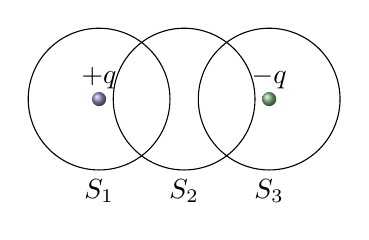
\begin{tikzpicture}[scale=.9]
        \shade [ball color=MidnightBlue!50] (-1.2,0) circle (.1);
        \shade [ball color=DarkGreen!50] (1.2,0) circle (.1);
        \draw (0,0) circle (1);
        \draw (-1.2,0) circle (1);
        \draw (1.2,0) circle (1);
        \node [anchor=south] at (-1.2,0) {$+q$};
        \node [anchor=south] at (1.2,0) {$-q$};
        \node [anchor=north] at (-1.2,-1) {$S_1$};
        \node [anchor=north] at (0,-1) {$S_2$};
        \node [anchor=north] at (1.2,-1) {$S_3$};
    \end{tikzpicture}\vspace*{\fill}
\end{problem}\switchcolumn
\solute2
\begin{solution}
    $S_1$内有电荷$q$，$S_2$内没有电荷，$S_3$内有电荷$-q$. 由高斯定理得三个闭合曲面的电通量分别为$q/\epsilon_0$，$0$，$-q/\epsilon_0$.
\end{solution}
\end{paracol}

\begin{paracol}{2}
    \begin{problem}
        质量分别为$m$和$2m$的两物体（都可视为质点），用一长为$l$的轻质刚性细杆相连，系统绕通过杆且垂直的竖直固定轴$O$转动，已知$O$轴离质量为$2m$的质点的距离为$l/3$，质量为$m$的质点的线速度为$v$且与杆垂直，则该系统对转轴的角动量大小\ans{$mvl$}.
        \switchcolumn\vspace*{\fill}\centering
        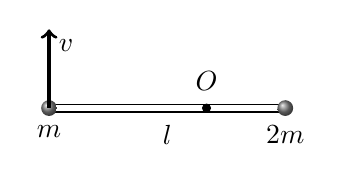
\begin{tikzpicture}
            \draw (0,-.05) -- (3,-.05) -- (3,.05) -- (0,.05)--cycle;
            \shade [ball color=gray] (0,0) circle (.1);
            \shade [ball color=gray] (3,0) circle (.1);
            \draw [very thick,->] (0,0) -- (0,1);
            \node [anchor=west] at (0,.8) {$v$};
            \filldraw (2,0) circle (.05);
            \node [anchor=north] at (0,-.1) {$m$};
            \node [anchor=north] at (1.5,-.1) {$l$};
            \node [anchor=north] at (3,-.1) {$2m$};
            \node [anchor=south] at (2,.1) {$O$};
        \end{tikzpicture}\vspace*{\fill}
    \end{problem}
\end{paracol}
\solute4\solute*{为节约资源，本试题计算题部分不提供演算区域，请自备稿纸，或在下页边缘书写.}
\begin{solution}
    系统角速度$\displaystyle\omega=v/(2l/3)=3v/2l$，角动量$L=I\omega=[m\cdot(2l/3)^2+2m\cdot(l/3)^2]\omega=mvl$.
\end{solution}

\section{计算题（共52分）}

\begin{problem}
    一半径为$\qty{20}\cm$的圆柱体，可绕与其中心轴线重合的光滑固定轴转动. 圆柱体上绕上绳子. 圆柱体初角速度为零，现拉绳的端点，使其以$\qty2{\m\cdot\s^{-2}}$的加速度运动. 绳与圆柱表面无相对滑动. 试计算在$t=\qty3\s$时
    \begin{tasks}[label=\arabic*.](2)
        \task 圆柱体的角加速度.
        \task 圆柱体的角速度.
    \end{tasks}
\end{problem}
\begin{solution}\leavevmode
    \begin{tasks}[label=\arabic*.](2)
        \task $\beta=a/r=\qty{10}{\radian\cdot\s^{-2}}$.
        \task $\omega=\omega_0+\beta t\big|_{\omega_0=0,t=\qty3\s}=\qty{30}{\radian\cdot\s^{-2}}$
    \end{tasks}
\end{solution}

\begin{paracol}{2}
\begin{problem}
    一半径为$R$、转动惯量为$I$的圆柱体$B$，可绕水平固定的中心轴$O$无摩擦地转动. 起初圆柱体静止，一质量为$M$的木块以速度$v_1$在光滑水平面上向右滑动，并擦过圆柱体的上表面跃上另一同高度的光滑表面，如图. 设它和圆柱体脱离接触前，它们之间无相对滑动. 试求木块的最后速率$v_2$.
    \switchcolumn\vspace*{\fill}\centering
    \begin{tikzpicture}[scale=.75]
        \draw [very thick,line cap=butt] (-2.8,0) -- (-.8,0) -- (-.8,-1.8);
        \fill [pattern=north east lines] (-2.8,0) rectangle (-.8,-.3) rectangle (-1.1,-1.8);
        \draw [very thick] (2.8,0) -- (.8,0) -- (.8,-1.8);
        \fill [pattern=north east lines] (2.8,0) rectangle (.8,-.3) rectangle (1.1,-1.8);
        \draw (0,-.5) circle (.5) node [left] {$\scriptscriptstyle O$} node [above] {$\scriptscriptstyle B$} -- (0,-1);
        \fill (0,-.5) circle (.05);
        \draw (-1.3,0) rectangle (-2,.5) node [midway] {$\scriptstyle M$};
        \draw [very thick,->] (-1.9,.75) -- (-1.4,.75) node [near end,above] {$\scriptstyle\bm v_1$};
        \draw [dashed] (1.3,0) rectangle (2,.5);
        \draw [very thick,->] (1.4,.75) -- (1.9,.75) node [near end,above] {$\scriptstyle\bm v_2$};
    \end{tikzpicture}
\end{problem}
\end{paracol}
\begin{solution}
    由物块和圆筒对$O$点角动量守恒得$mv_1R=mv_2R+I\omega$. 擦过圆柱体的过程中，二者之间无相对滑动，代入纯滚动约束$v=\omega R$得$v_2=mv_1R^2/(I+mR^2)$.
\end{solution}

\begin{paracol}{2}
\begin{problem}
    如图所示，质量为$m_2$的物体与轻弹簧相连，弹簧另一端与一个质量可忽略的挡板连接，静止在光滑的桌面上. 弹簧劲度系数为$k$. 今有一质量为$m_1$，速度为$\bm v_0$的物体向弹簧运动并与挡板正碰，求弹簧最大的被压缩量.
    \switchcolumn\vspace*{\fill}\centering
    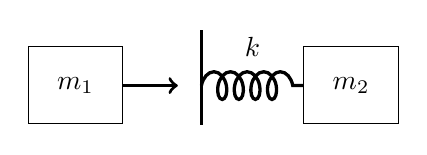
\begin{tikzpicture}
        \wall{(-2.5,0)}{(2.5,-.2)};
        \draw (-2.2,.02) rectangle (-1,1);
        \draw [very thick,->] (-1,.5) -- (-.3,.5);
        \draw [very thick] (0,0) -- (0,1.2);
        \draw (1.3,.02) rectangle (2.5,1);
        \draw [very thick,decoration={aspect=.6, segment length=6, amplitude=5,coil},decorate] (0,.5) -- (1.3,.5); %amplitude调整螺线管的直径，segment length调整间距
        \node at (-1.6,.5) {$m_1$};
        \node at (1.9,.5) {$m_2$};
        \node [above] at (.65,.75) {$k$};
    \end{tikzpicture}\vspace*{\fill}
\end{problem}
\end{paracol}
\begin{solution}
    刚碰撞后$m_1$的速度大于$m_2$，弹簧不断压缩. 当$m_1$和$m_2$共速时，弹簧压缩量最大，弹性势能最大. 物块、弹簧、挡板组成的系统在水平方向上动量守恒和系统机械能守恒可分别列出
    \[\begin{dcases}
        m_1v_0=(m_1+m_2)v\\
        \frac12m_1v_0^2=\frac12(m_1+m_2)v^2+E_p
    \end{dcases}\]
    联立得弹簧的最大弹性势能为$E_p=m_1m_2v_0^2/2(m_1+m_2)$. 根据弹簧弹性势能表达式$E_p=k\Delta x^2/2$得弹簧的最大压缩量$\Delta x_{\max}=v_0\sqrt{m_1m_2/k(m_1+m_2)}$.
\end{solution}

\begin{paracol}{2}
\begin{problem}
    如图，一质点做半径$R=\qty4\m$的圆周运动，$t=0$时质点位于$A$点，然后顺时针方向运动，运动方程$S=\pi t^2+2\pi t$ (SI). 求
    \begin{enumerate}
        \item 质点绕行一周所经历的路程、位移、平均速率.
        \item 质点在$\qty1\s$末的速度和加速度的大小.
    \end{enumerate}
    \switchcolumn\vspace*{\fill}\centering
    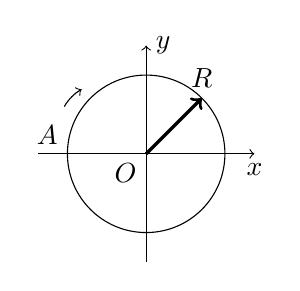
\begin{tikzpicture}[scale=.5]
        \draw (0,0) circle (2) node [below left] {$O$};
        \draw [->] (-2.75,0) -- (2.75,0) node [below] {$x$};
        \draw [->] (0,-2.75) -- (0,2.75) node [right] {$y$};
        \draw [->] (-2.08,1.2) arc (150:120:1.2);
        \node [anchor=south east] at (-2,0) {$A$};
        \draw [very thick,->] (0,0) -- ({sqrt(2)},{sqrt(2)}) node [above] {$R$};
    \end{tikzpicture}\vspace*{\fill}
\end{problem}
\end{paracol}
\begin{solution}\leavevmode
    \begin{enumerate}
        \item 质点绕行一周后回到起点，位移为零. 质点绕行一周，经历路程$\Delta S=2\pi R=8\pi\unit\m$. 令$S=\Delta S$得用时$\Delta t=\qty2\s$. 所以平均速率$\overline{v}=\Delta S/\Delta t=4\pi\unit{\m/\s}$.
        \item
        \begin{tasks}[label=\labelitemii](2)
            \task! 质点的速度大小$v=\d s/\d t=2\pi t+2\pi\big|_{t=\qty1\s}=4\pi\unit{\m/\s}$.
            \task 切向加速度$a_\tau=\d v/\d t=2\pi\unit{\m/\s}$.
            \task 法向加速度$a_n=v^2/R=4\pi^2/2\unit{\m/\s^2}$.
            \task! 所以质点的加速度为$a=\sqrt{a_{\tau}^2+a_n^2}=\qty{39.98}{\m\cdot\s^{-2}}$.
        \end{tasks}
    \end{enumerate}
\end{solution}

\begin{problem}
    质量为$m=\qty{4.8}\g$的子弹$A$，以$v_0=\qty{450}{\m/\s}$的速率水平地射入一静止在水平面上的质量为$M=\qty2\kg$的木块$B$内，$A$射入$B$后，$B$向前移动了$L=\qty{80}\cm$后而停止，求
    \begin{tasks}[label=\arabic*.](2)
        \task $B$与水平面间的摩擦系数$\mu$.
        \task 木块对子弹所做的功$W_1$.
        \task 子弹对木块所做的功.
    \end{tasks}
\end{problem}
\begin{solution}\leavevmode
    \begin{enumerate}
        \item 由子弹和木块系统动量守恒、入射后到减速至静止的过程动能定理分别有
        \[\begin{dcases}
            mv_0=(m+M)v\\
            -\mu(m+M)gl=\frac12(m+M)v^2
        \end{dcases}\]
        联立以上两式解得$\mu=0.074$.
        \item 木块对子弹所做的功等于碰撞前后子弹动能的增量$W_1=mv^2/2-mv_0^2/2=\qty{-486}\J$.
        \item 子弹对木块所做的功等于碰撞前后木块动能的增量$W_2=Mv^2/2=\qty{1.16}\J$.
    \end{enumerate}
\end{solution}

\begin{problem}
    两个均匀带电的同心球面，分别带有净电荷$q_1$和$q_2$，其中$q_1$为内球的电荷. 两球之间的电场为 $1500/r^2$ (SI)，且方向沿半径向外；球外的场强为$2000/r^2$ (SI)，方向沿半径向里，试求$q_1$和$q_2$各等于多少？（真空介电常数$\epsilon_0=\qty{8.85e12}{\C^2\N^{-1}\m^2}$）.
\end{problem}
\begin{solution}
    以沿半径向外为正方向，在两个球面的中间和外球面外侧取半径分别为$r_1$和$r_2$与球面同心的的高斯面. 由高斯定理
    \[E_1\cdot 4\pi r_1^2=q_1/\epsilon_0,\ E_2\cdot 4\pi r_2^2=(q_1+q_2)/\epsilon_0\]
    代入$E_1=1500/r_1^2$，$E_2=-2000/r_2^2$得$q_1=\qty{1.67e-7}\C$，$q_2=\qty{-3.89e-7}\C$.
\end{solution}

\begin{paracol}{2}
\begin{problem}
    图中虚线所示为一立方形的高斯面，已知空间的场强分布为$E_x=bx$，$E_y=0$，$E_z=0$. 高斯面边长$a=\qty{0.1}\m$，常量$b=\qty{1000}{\N/(\C\cdot\m)}$. 试求该闭合面中包含的净电荷（真空介电常数$\epsilon_0=\qty{8.85e12}{\C^2\N^{-1}\m^2}$）.
    \switchcolumn\vspace*{\fill}\centering
    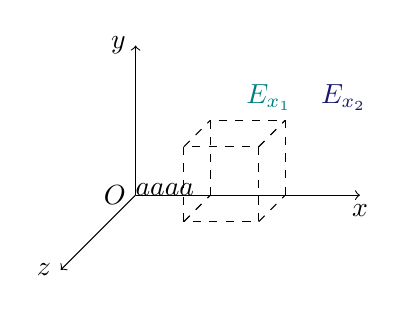
\begin{tikzpicture}[scale=.95]
        \draw [->] (0,0) node [left] {$O$} -- (0,2) node [left] {$y$};
        \draw [->] (0,0) -- (3,0) node [below] {$x$};
        \draw [->] (0,0) -- (-1,-1) node [left] {$z$};
        \draw [dashed] (1,0) rectangle (2,1);
        \draw [dashed,xshift=-.25*sqrt(2)*1cm,yshift=-.25*sqrt(2)*1cm] (1,0) rectangle (2,1);
        \draw [dashed] ({1-.25*sqrt(2)},{1-.25*sqrt(2)}) -- (1,1) ({2-.25*sqrt(2)},{1-.25*sqrt(2)}) -- (2,1);
        \draw [dashed] ({1-.25*sqrt(2)},{-.25*sqrt(2)}) -- (1,0) ({2-.25*sqrt(2)},{-.25*sqrt(2)}) -- (2,0);
        \length{({-.25*sqrt(2)},{-.5*sqrt(2)})}{({1-.25*sqrt(2)},{-.5*sqrt(2)})}{$a$}{(.5,0)};
        \length{({1-.25*sqrt(2)},{-.5*sqrt(2)})}{({2-.25*sqrt(2)},{-.5*sqrt(2)})}{$a$}{(.5,0)};
        \length{({2.25-.25*sqrt(2)},{-.25-.25*sqrt(2)})}{(2.25,-.25)}{$a$}{({.5*sqrt(2)},{.5*sqrt(2)})};
        \length{(2.4,0)}{(2.4,1)}{$a$}{(0,.5)};
        \node [teal,anchor=south] at (1,1) {$\bm E_{x_1}$};
        \node [MidnightBlue,anchor=south] at (2,1) {$\bm E_{x_2}$};
    \end{tikzpicture}\vspace*{\fill}
\end{problem}
\switchcolumn
\begin{solution}
    高斯面的左、右表面电通量分别为$E_{x_1}a^2$，$E_{x_2}a^2$，其余表面电通量均为零. 由高斯定理
    \switchcolumn*[\noindent %
    \[(E_{x_2}-E_{x_1})a^2=(ba-2ba)a^2=Q/\epsilon_0\]
    得$Q=\epsilon ba^3=\qty{8.85e-12}\C$.]
\end{solution}
\end{paracol}